\section{Experimental Results}\label{sec:results}

In this section, we present the experimental results according to our four research questions (RQs).

\subsection*{\textbf{(RQ1) \rqone}}

% \kla{Wannita, please compute the \% in the blank throughout the paper. Thanks.}


% Compare results to the state-of-the-art baselines. \kla{will check again after the table is revised. PyCoder to the top, sort from max to min. Double-check capitalization carefully, Make it neat, fits the table nicely to the column. add batch size column too. }


\indent \textbf{\our.} Among our comprehensive investigation, the best setting for \our~is to train with the hard parameter sharing strategy (\our-Hard), a task weight of 9:1 (code:type) using a Beam Search as a decoding method.
We use this setting as a reference for comparison with other approaches throughout the paper.

% \noindent \textbf{Results.} 
\textbf{\our~achieves the first rank on the CodeXGLUE leaderboard for the code completion task} (as of 13 October 2022, see Table~\ref{tab:rq1 codexglue}).
% \kla{ in the website, it shows line first, then token. for our case, there is a bigger improvement for line, than token. why don't we sell line first, then token? thought?}
We find that \our~achieves an accuracy of 76.93\% for the token-level predictions, while achieving an exact match of 43.91\% for the line-level predictions.
The evaluation results confirm that  \our~is more accurate than other baselines by 0.43\%-24.25\% for token-level predictions and 3.63\%-84.73\% for line-level predictions.
% \kla{may talk about why small improvement - could be due to batch size, limited GPU capacity, etc... at least, still outperform and}

Similarly, \textbf{\our~outperforms existing AST-based and non-AST-based code completion approaches}, according to our own setting.
Table~\ref{tab:rq1 our} shows that \our~achieves an accuracy of 77.12\% for the token-level predictions, while achieving an exact match of 43.37\% for the line-level predictions.
For the token-level predictions (Acc), we find that \our~is more accurate than Pointer Mixture Network by 11.74\%, GPT-2 by 4.37\%, TravTrans by 2.15\%, and CodeGPT by 1.89\%. 
This finding indicates that \our~that is syntax-aware and on-the-fly performs better than a code completion approach that is either syntax-aware alone or on-the-fly alone.
It is worth noting that the accuracy of \our-Hard, CodeGPT, and GPT-2 achieved for the CodeXGLUE leaderboard is slightly different from the accuracy of those that are run in our experimental setup.
The difference that we observed has to do with the dataset used in CodeXGLUE and our experiment.
In CodeXGLUE, they removed the indentation, while the dataset used in our experiment preserved the original indentation.
To mimic the practical deployment scenario, we opt to preserve the original indentation.

% \kla{will talk about the small diff value btw codexglue and our own here why}

In addition, \textbf{the token-type information can improve the line-level code completion task by 8.34\%-15.22\%.}
For the line-level predictions (EM), we find that \our~is more accurate than GPT-2 by 15.22\% and CodeGPT by 8.34\%. 
This finding indicates that the use of token-type information that is largely ignored by the literature can also improve the line-level predictions by 8.34\% to 15.22\%, confirming that the token-type information is useful to improve the performance of line-level code completions.

Finally, when comparing \our~with the existing AST-based code completions (i.e., TravTrans and Pointer Mixture Network), we find that the existing AST-based code completions are designed for the token-level predictions only.
Thus, the line-level predictions cannot be performed, highlighting the limitations of the AST-based approaches that require AST information at the inference time, while demonstrating the benefits of our approach that consider the token-type information (i.e., \emph{syntax-aware}), while can still predict code at any points of time (i.e., \emph{on-the-fly}).


% We evaluate the performance of our SynComp to complete the source code in token-level prediction and line-level prediction, compare against 4 state-of-the-art baselines and CodeXGLUE benchmark.
% \kla{do XXX.}
% We have two main results in this research question. 
% First is the results of \our~comparing with four state-of-the-art approaches implementing from their replication packages.
% Second is the results we receive from CodeXGLUE benchmark~\cite{lu2021codexglue} on code completion task.


% \our~model used in this RQ is PyCoder-Hard i.e., the MTL: hard parameter sharing with task's weight 9:1 (code:type) model which give the best experimental results from RQ~2~to~4.
% Below we provide the details of our results.

% \kla{will go from here once the table is revised.}

% \textbf{\our~on CodeXGLUE Benchmark} 
%     In Table.~\ref{tab:rq1 codexglue} shows the results of \our~in code completion task on CodeXGLUE benchmark\footnote{https://microsoft.github.io/CodeXGLUE/}.
%     Note that we run our \our~on CodeXGLUE dataset and send the predictions to CodeXGLUE benchmark for evaluation.
%     The results validate that our \our~surpasses the state-of-the-art CodeGPT and CodeGPT-adapt model, resulting in the first place in CodeXGLUE's python code completion tasks.
%     Specifically, in token-level prediction, the accuracy is relatively improved by 0.43\% %0.33\% 
%     (from 76.60 to 76.93).
%     While in line-level predictions, the exact match is relatively improved by 3.73\% %1.58\% 
%     (from 42.37 to 43.91) and the edit similarity is relatively improved by 0.21\% %0.15\% 
%     (from 71.59\% to 71.74\%).

    
% \textbf{\our~with State-of-the-art approaches} 
%     In Table.~\ref{tab:rq1} shows the results of \our~with four state-of-the-art approaches: Pointer Mixture Network~\cite{li2017code}, TravTrans~\cite{kim2021code}, GPT-2~\cite{radford2019language}, and CodeGPT~\cite{lu2021codexglue}.
%     % All state-of-the-art approaches are run from their replication packages and fine-tuning with the best hyperparameters reported in their papers.
%     The results show that our model surpass all state-of-the-art approaches.
%     Compared with second-best models, \our~achieves an improvement on accuracy of 1.89\% (from 75.69\% to 77.12\%) in token-level prediction, and on exact match of 8.34\% (from 40.03\% to 43.37\%) and edit similarity of 3.67\% (from 70.61\% to 73.20\%) in line-level prediction.
    % In token-level prediction, the accuracy is relatively improved by 1.89\% %1.43\% 
    % (from 75.69\% to 77.12\%). 
    % In line-level completion, the Exact Match is relatively improved by 8.34\% %3.34\% 
    % (from 40.03\% to 43.37\%) and edit similarity is relatively improved by 3.67\% % 2.59\% 
    % (from 70.61\% to 73.20\%). 

    

% \begin{itemize}
%     \item 

    
%     \item 
% \end{itemize}

% As a result, this can indicate that the token type syntactic information can be beneficial as a supporting data and does help enhance the performances in both token-level and line-level code completion.

% diff due to
% dataset — table3 (our) keep indentation info. , table4(codexglue) discard indentation info.
% batch size — table 4 no batch size information, but what is our?


\begin{tcolorbox}

% To answer this RQ, we build SynComp from the best combination of experiments on model technique (RQ2), task weighing parameters (RQ3) and decoding methods (RQ4) i.e. hard parameters sharing model with weighing code to type tasks as 9:1, and beam search as decoding methods.See the details of each experiment result in the following RQs.
\emph{\textbf{RQ1 Summary.} 
\fdone
% \our~surpasses all the state-of-the-art code completion models.
% The line-level exact match is improved by 8.34\%-15.22\%, while the token-level accuracy is improved by 1.89\%-11.74\%.
% \our~also receives the first place in CodeXGLUE’s python code completion benchmark. The results indicate that the token type syntactic information can be beneficial as a supporting data.
}
\end{tcolorbox}

% \subsection{RQ2: What is the impact of the training strategies on the performance of our approach}
\begin{table}[t]
    \centering
    % \resizebox{\columnwidth}{!}{
    \begin{tabular}{l|c|c|c|c}
        & \multicolumn{3}{c}{Line-level} & \multicolumn{1}{|c}{Token-level}\\
        \hline
        Model & EM & ES & MRR & Acc \\%& Type Acc \\
        \hline
        \our-Hard & \textbf{42.83} & \textbf{72.82} & 48.42 & \textbf{77.00} \\ %& \textbf{82.49} \\
        \our-IFN & 42.04 & 71.92 & \textbf{48.54} & 76.52 \\ %& 0.0 \\
        \our-Soft & 38.29 & 69.11 & 44.66 & 74.77 \\ %& 80.68 \\
    \end{tabular}
    % }
    \caption{(RQ2) The results of \our~when using various multi-task training strategies. For a fair comparison with other multi-task training strategies, we do not put any weights between tasks on \our-Hard (i.e., \emph{No Weight}).
    % \kla{I feel type acc should be dropped. irrelevant, and never talked about it before.}
    }
    \label{tab:rq2}
\end{table}

% To answer this research question, we compare the best results of each model techniques after tuning weighing (see session 5.3). The results are shown in Table \ref{tab:rq2}. From the table, hard parameters sharing with manual weight of 9:1 perform the best in both token-level and line-level prediction. This is also the method we decide to use sending results to CodeXGLUE competition. Second place is \gls{ifn} method. Even though \gls{ifn} method give comparable results to hard parameters sharing model. When we train further to the optima, the \gls{ifn} model are struggled on forgetting catastrophe \cite{} which cause the model to perform worse than hard parameters sharing later.   

% if no-weight results -> write about even if IFN is slightly better but when training further the results drop because of the forget catastrophe

% \textbf{Approach.} To answer this research question, we compare the results of each model training techniques: hard parameters sharing (MTL), soft parameters sharing (MTL), and intermediate fine-tuning (STILTs); before tuning the task weighing parameters. 

\subsection*{\textbf{(RQ2) \rqtwo}}

Table~\ref{tab:rq2} presents the results of \our~when using various multi-task training strategies.

\textbf{Hard parameter sharing (\our-Hard) as a multi-task training strategy performs the best.}
Table~\ref{tab:rq2} shows that different multi-task training strategies have an impact on the performance of \our~for both token-level and line-level predictions.
Particularly, we observe that \our~with hard parameter sharing achieves an exact match of 42.83\%, while \our~with software parameter sharing achieves an exact match of 38.29\%. 
The 4.54\% difference (i.e., max-min) confirms the impact that the training strategies have on the performance of \our.
In addition, our results are contradictory to Izadi~\ea~\cite{izadi2022codefill} who found that soft parameter sharing performs best for code completion.
% , while being in line with Liu~\ea~\cite{liu2022unified} who found that hard parameters sharing performs best.
This finding highlights the importance of investigating various choices of multi-task training strategies for code completions, instead of following prior suggestions or practices.

Different from Izadi~\ea~\cite{izadi2022codefill}, our \our-Hard is designed to take both sequences of code tokens and their types as inputs one-by-one at a time and simultaneously learn with the same loss functions that are optimized together within the same model.
With this method, the inputs can be detached from each other at the inference phase, resulting in better performance confirmed by our results.
Nonetheless, the high-performing hard parameter-sharing training strategy (\our-Hard) has to do with the benefits of the tight relationship between the learning tasks (i.e., code predictions and type predictions).
Since token types are directly aligned with the same sequence of code tokens, these two pieces of information have a tight relationship.
Therefore, \our-Hard, which completely shares the model’s weights and parameters between tasks, gains the most benefit from the shared relationship between the code and type information.
However, the soft parameter sharing model (\our-Soft) learns each task separately, making the learning process between two related tasks harder, resulting in sub-optimal performance.

% Our \our-Hard~is designed to take both sequences of code tokens and their types as input and simultaneously learn with the same loss functions that are optimized together within the same model.
% With this method, the model will be able to learn the syntactic information from types in the training phase without requiring types in the inference phase as the inputs can be detached from each others.
% The results in Tables~\ref{tab:rq2} show that this hard parameter sharing model -- \our-Hard performs the best in our case.
% \kla{why this is great?}

% Our \our-IFN~is designed to learn all sequence of types and then code tokens separately. 
% Thus, similar to \our-Hard, \our-IFN  is also able to predict without types in the inference phase as the tasks are learnt separately but sequentially within the same model.
% The results in Table~\ref{tab:rq2} show that this intermediate fine-tuning model -- \our-IFN performs as the second place in our case.
% However, we observed the type accuracy in token-level prediction and found that type accuracy of \our-IFN go down to 0\%.
% As a results, it shows that the model faces prevalent problems when training a model sequentially: a catastrophic forgetting~\cite{mccloskey1989catastrophic, kaushik2021understanding}.
% In other words, \our-IFN has already forgotten the token type information which is the reason of the worse results than \our-Hard which can access the type data all along the training.

% Our \our-Soft~is designed to take sequences of code tokens and types to learn in separated models, then optimizes simultaneously with the loosely joint to share knowledge between the models.
% Therefore, although being trained together, the model can be used separately in the inference phase allowing the prediction without type inputs.
% The results in Table~\ref{tab:rq2} show that the soft parameter sharing model -- \our-Soft performs as the last in our case.

% \kla{need to discuss/explain why hard is better than soft, why soft is worst?}

% \textbf{Results.} 
% The results are presented in Table~\ref{tab:rq2}.
% indicating that the different multi-task training techniques can vary the results as follows.
% In token-level prediction, the accuracy can be relatively different by 2.98\% %2.23\%
% (from 74.77\% to 77.00\%), and in line-level prediction, the exact match is relatively different by 11.86\% %4.54\% 
% (from 38.29\% to 42.83\%), the edit similarity by 5.37\% %3.71\%
% (from 69.11\% to 72.82\%) and the mean reciprocal rank by 8.69\% %3.88\% 
% (from 44.66\% to 48.54\%).
% In particular, we can observe that the best multi-task training technique in our setting is the \emph{MTL: hard parameters sharing model} (\our-Hard), which give the highest score in both token-level prediction (accuracy=77.00\%) and line-level prediction (exact match=42.83\%).
% This is contrast to a recent study of Izadi~\ea\cite{izadi2022codefill} which propose CodeFill with soft parameters sharing model over hard parameters sharing model.

% However, it is worth noting that different from CodeFill which the input is the concatenation of type and token, our hard parameters sharing model feeds inputs separately while optimizing together.
% On the contrary, the worst model are the \emph{MTL: soft parameters sharing model} (\our-Soft), which in this comparison give the lowest scores in both token-level prediction (accuracy=74.77\%) and line-level prediction (exact match=38.29\%).
% The explanation for these gaps might be because the token type information is a lot correspondent to the source code from which the types directly extracted and aligned in sequences.
% Thus, the hard parameters sharing model, which completely shares the model's weights and parameters between tasks, is reasonable improving the performance; however, the soft parameters sharing model which learn each task separately might be more struggle to relate the tasks.

% Additionally, we also show the accuracy of token-level prediction for token types in Table.~\ref{tab:rq2} which clearly emphasizes the different between MTL and IFN. 
% Even though the results of IFN model for code completion is comparable to the one produced by hard parameters sharing model with difference by 0.63\% (from 76.52\% to 77.00\%) in the token-level prediction accuracy and 1.88\% (from 42.04\% to 42.83\%) in the line-level prediction exact match, we can observe that the IFN \emph{type} prediction accuracy is go down to 0\%.
% As IFN model is fine-tuned firstly on type prediction (supporting task), then fine-tuned on code prediction (target task); thus, this could cause the prevalent problems when training a model sequentially: a catastrophic forgetting~\cite{mccloskey1989catastrophic, kaushik2021understanding}.
% As a result, the IFN model has already forgotten the token type information which is the reason of the worse results than hard parameters sharing model that can access the supporting data all along the training.

% From the table, hard parameters sharing model perform the best in both token-level and line-level prediction. This is also the method we decide to use sending results to CodeXGLUE benchmark. Second place is \gls{ifn} method. Even though \gls{ifn} method give comparable results to hard parameters sharing model, by observing to type prediction results, we can see that the model are struggled on catastrophic forgetting~\cite{kaushik2021understanding}. 
% This may cause the model to perform worse than hard parameters sharing which can access the auxiliary data all along the training.

\begin{tcolorbox}
\emph{\textbf{RQ2 Summary.}} 
\fdtwo

% highlights the importance of investigating various choices of multi-task training strategies for code completions, instead of following prior suggestions or practices

% The best multi-task training technique for our setting is \our-
% IFN: Intermediate Fine-tuning (\our-IFN) and MTL: Soft Parameter Sharing (\our-Soft).
% Particularly, the exact match in line-level prediction is vary by 4.54\%.

\end{tcolorbox}

\subsection*{\textbf{(RQ3) \rqthree}}
% \subsection{RQ3: What is the impact of the task weighting parameters in multi-task learning on the performance of our approach?}
% \begin{table}[]
%     \centering
%     \begin{tabular}{l|c|c|c|c|c}
%         Model & Code Acc & Type Acc & \gls{em} & \gls{es} & \gls{mrr} \\
%         \hline
%         Random & & & & &\\
%         Random with control & & & & &\\
%         Manual 7:2:1 & & & & &\\
%     \end{tabular}
%     \caption{The sensitivity of weighing for soft parameters sharing model performances.}
%     \label{tab:rq3 soft-share}
% \end{table}

\begin{table}[t]
    \centering
    % \resizebox{\columnwidth}{!}{
    \begin{tabular}{l|c|c|c|c}
        Task's Weight & \multicolumn{3}{c}{Line-level} & \multicolumn{1}{|c}{Token-level}\\
        \hline
        Type:Code & EM & ES & MRR & Acc \\ %& Type Acc \\
        \hline
        No Weight & 42.83 & 72.82 & 48.42 & 77.00 \\% & 82.49 \\
        1 : 9 & \textbf{43.37} & \textbf{73.20} & 48.82 & \textbf{77.12} \\ %& 81.16 \\
        2 : 8 & 43.08 & 73.01 & 48.73 & \textbf{77.12} \\ %& 81.72 \\
        3 : 7 & 42.95 & 72.94 & 48.56 & 77.10 \\% & 82.05 \\
        4 : 6 & 42.84 & 73.03 & 48.55 & 77.05 \\% & 82.29 \\
        5 : 5 & 42.94 & 72.69 & \textbf{49.53} & 76.99 \\% & 82.47 \\
        6 : 4 & 42.37 & 72.29 & 49.10 & 76.88 \\% & 82.65 \\
        7 : 3 & 42.28 & 72.27 & 47.82 & 76.70 \\% & 82.77 \\
        8 : 2 & 41.19 & 71.68 & 46.76 & 76.23 \\% & 82.75 \\
        9 : 1 & 39.77 & 70.52 & 46.34 & 75.45 \\% & \textbf{82.83}
        
        % 1 : 9 & 39.77 & 70.52 & 46.34 & 75.45 & \textbf{82.83} \\
        % 2 : 8 & 41.19 & 71.68 & 46.76 & 76.23 & 82.75 \\
        % 3 : 7 & 42.28 & 72.27 & 47.82 & 76.70 & 82.77 \\
        % 4 : 6 & 42.37 & 72.29 & 49.10 & 76.88 & 82.65 \\
        % 5 : 5 & 42.94 & 72.69 & \textbf{49.53} & 76.99 & 82.47 \\
        % No Weight & 42.83 & 72.82 & 48.42 & 77.00 & 82.49 \\
        % 6 : 4 & 42.84 & 73.03 & 48.55 & 77.05 & 82.29 \\
        % 7 : 3 & 42.95 & 72.94 & 48.56 & 77.10 & 82.05 \\
        % 8 : 2 & 43.08 & 73.01 & 48.73 & \textbf{77.12} & 81.72 \\
        % 9 : 1 & \textbf{43.37} & \textbf{73.20} & 48.82 & \textbf{77.12} & 81.16 \\
        % 9.5 : 0.5 & 43.31 & 73.12 & 48.87 & \textbf{77.12} & 80.61 \\
    \end{tabular}
    % }
    \caption{(RQ3) The results of different task weighing parameters for Hard Parameter Sharing only as \our-Hard performs best.}
    \label{tab:rq3 hard-share}
\end{table}

% \textbf{Approach.} To answer this research question, we choose the hard parameters sharing model to experiment on the weighing sensitivity as it is the best model from RQ2. We manually tune the model with different weights according to equation~\ref{eq:rq3} where $\alpha$ is the weight.

% \textbf{Results.} 
Table~\ref{tab:rq3 hard-share} presents the results of different task weighing parameters for \our-Hard.

\textbf{\our~is generally robust to the task weighting parameters, achieving comparative (without task weighting) or better (with task weighting) performance when compared to the baselines.}
Table~\ref{tab:rq3 hard-share} shows that when varying the task weighting parameters (Type:Code) from 1:9 to 9:1, our \our~achieves an exact match between 41.19\% to 43.37\%, which is still greater than the existing approaches (i.e., 40.03\% for CodeGPT and 37.64\% for GPT-2) with an exception for the weighting of 9:1.
Although the task parameters are not weighted (cf. \emph{No Weight}), our \our~still achieves an exact match of 42.83\%, which also outperforms the existing approaches.
In line with the other measures for both line-level and token-level predictions, this finding confirms that by adding token-type information by at least a small weighting of 10\%, our \our~often performs better than the existing approaches.
% \kla{need to mention the gradient thing}
This means that the task objectives of \our~rarely suffered from conflicting gradients (i.e., the gradients of different task objectives are not aligned leading to the sub-optimal performance in the average gradient) showing that type prediction and code prediction are correspondent and beneficial to each other.
In our setting, the best task's weight is 1:9 for the type prediction task to the code prediction task.

% The results is shown in Table.~\ref{tab:rq3 hard-share}. 
% Note that due to the resource limitation, we perform this RQ experiments only on hard parameters sharing model as it is the technique that give the best performance from experiments in RQ2.
% The results show that the task weighing parameters do impact \our~performance.
% In fact, when adjusting the weights, the accuracy in token-level prediction can be relatively vary by 2.21\% %1.67\% 
% (from 75.45\% to 77.12\%).
% In line-level prediction, the exact match, edit similarity and mean reciprocal rank can be relatively vary by 9.05\% %3.6\% 
% (from 39.77\% to 43.37\%), 3.80\% %2.68\% 
% (from 70.52\% to 73.20\%) and 6.88\% %3.19\% 
% (from 46.34\% to 49.53\%) respectively.
% On the other hand, if comparing to the model without task weighing parameters, all the performance are slightly increased when adjusting the weights:
% in token-level prediction the accuracy is relatively boosted up by 0.16\% %0.12\% 
% (from 77.00\% to 77.12\%), and
% in line-level prediction the exact match, edit similarity and mean reciprocal rank are relatively boosted up by 1.26\% %0.54\% 
% (from 42.83\% to 43.37\%), 0.52\% %0.38\% 
% (from 72.82\% to 73.20\%) and 2.29\% %1.11\% 
% (from 48.42\% to 49.53\%).

% Thus, the study also shows that \our~is rarely suffered from the conflicting gradients which could be because of the model trained on two very similar tasks.
% This can yield to the conclusion that \our~is robust to the task weighing parameters and can also perform well without weighing; additionally, the model can perform slightly better in both level predictions when tuning the task weighing parameters.

% To our setting, the best task's weight is 9:1 for code prediction task to type prediction task.
% We choose this weight combination for predicting results to compete with state-of-the-art approaches and CodeXGLUE benchmark.

\begin{tcolorbox}
\emph{\textbf{RQ3 Summary.}
\fdthree{}
% The results show that \our~is robust to the task weighing parameters; additionally, the model can perform slightly better in both level predictions when tuning the weights.
% The best task’s weight for our work is 9:1 for code to type prediction task.
}
\end{tcolorbox}

\subsection*{\textbf{(RQ4) \rqfour}}
% \subsection{RQ4: What is the impact of the decoding methods on the performance of our approach?}
\begin{table}[t]
    \centering
    \resizebox{\columnwidth}{!}{
    \begin{tabular}{l|l|c|c}
        & & \multicolumn{2}{c}{Line-level} \\
        \hline
        Library & Method & EM & ES \\
        \hline
        \multirow{2}{*}{CodeXGLUE}
        & Beam Search ($b$=5) & \textbf{43.37} & 73.20 \\ 
        & Greedy & 41.47 & \textbf{73.95} \\ 
        \hline
        \multirow{6}{*}{HuggingFace}
        & Beam Search ($b$=5) & \textbf{41.52} & 72.85 \\
        & Greedy & 41.48 & 73.96 \\ 
        & Sampling & 33.80 (0.16) & 68.72 (0.11) \\ 
        & Sampling with Temp ($temp$=0.1) & 41.38 (0.10) & \textbf{73.98 (0.03)} \\ 
        & Top-K Sampling ($k$=3) & 35.34 (0.16) & 70.43 (0.11) \\ 
        & Top-P Sampling ($p$=0.1) & 41.48 (0.01) & 73.95 (0.01) \\
        
        % & Sampling & 33.80$\pm$0.07 & 68.72$\pm$0.05 \\ 
        % & Sampling with Temp ($temp$=0.1) & 41.38$\pm$0.04 & \textbf{73.98$\pm$0.01} \\ 
        % & Top-K Sampling ($k$=3) & 35.34$\pm$0.07 & 70.43$\pm$0.05 \\ 
        % & Top-P Sampling ($p$=0.1) & 41.48$\pm$0.01 & 73.95$\pm$0.01 \\
        
        % & Sampling & 33.68 & 68.60 \\ 
        % & Sampling with Temp ($temp$=0.1) & 41.49 & \textbf{74.01} \\ 
        % & Top-K Sampling ($k$=50) & 33.85 & 69.13 \\ 
        % & Top-P Sampling ($p$=0.1) & 41.48 & 73.97 \\ 
    \end{tabular}}
    \caption{(RQ4)  The results of different decoding methods for Hard Parameter Sharing (1:9). For any sampling methods, we report both the Mean and its standard deviation (SD).
    }
    \label{tab:rq4}
\end{table}

% To recommend code review comments, Com- mentFinder leverages the cosine distance to retrieve the ten nearest changed methods and GPM to identify the �� most similar changed methods. Although other distance and text similarity metrics are available, they may provide different results. Yet, little is known about the impact that these simi- larity techniques can have on the effectiveness and efficiency of our CommentFinder. Hence, we formulate this RQ to further investigate the possible impact when the distance metrics or text similarity metrics in CommentFinder are changed.

\begin{figure*}
    \centering
    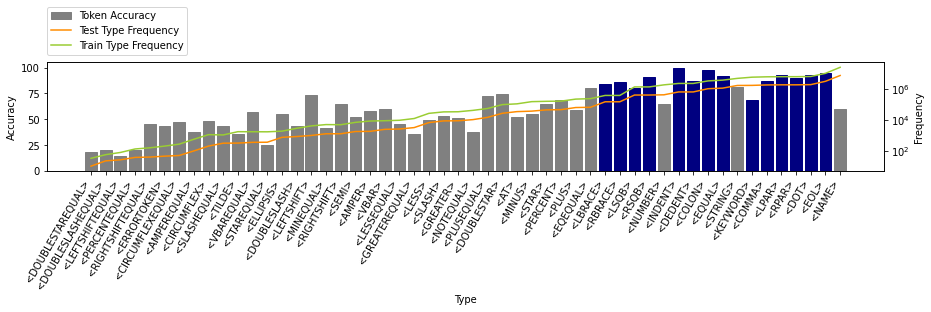
\includegraphics[width=\textwidth]{figures/pycoder_type_discussion_grammar.png}
    \caption{The chart of the token-level code prediction accuracy in token type granularity sorted by the type frequency from small (left) to large (right).}
    \label{fig:type_barplot}
\end{figure*}

% \textbf{Approach.} To answer this research question, we study the difference between following decoding methods. 

% \begin{itemize}
    \item \textbf{Greedy} is a method to select the maximum probable vocabulary to be the next tokens.
    This method assumes that the model already outputs the best probability in every timestep.
    % it generates all possible tokens in the vocabulary list; then, it will choose top B candidates that have the most probability. Those B candidates will move to the next time step, and the process repeats. In the end, there will only be B candidates. The search space is only (10,000)*B.
%     Although selecting only the highest
% probability token is suitable for a specific time step, it
% might be a sub-optimal for a sequence. 
    
    \item \textbf{Beam Search} applies a search algorithm to generate all possible tokens in the vocabulary; then, it selects the top $b$ (i.e., beam size) probable tokens to continue.
    The Beam Search method is one of the most commonly used decoding methods in text generation tasks~\cite{li-etal-2016-deep, wiseman-etal-2017-challenges}.
    % However, Beam Search may not always achieve optimal results, since it does not consider the whole vocabulary, but instead only the top $b$ (i.e., beam size) probable tokens.
    % Nevertheless, Beam Search still performs faster than an exhaustive search.
    
    % ; however, it balances between the performance and the computational time.
    % The method's time complexity is equals to $O(b*V)$ where $V$ is the vocabulary size.
    % It . 
    
    % recommend the most probable $b$ next tokens according to a defined $b$ beam size threshold.

    
    
    
    % by expanding the graph in a limited set called beam~size~($b$).
    % In each timestep, the method generates all possible tokens in the vocabulary; then, it select the top $B$ probability tokens to continue.
      
    
    \item \textbf{Sampling} is a method to randomly select the next token from the actual probability distribution assigned by the model.
    Different from Greedy and Beam search methods which in some cases may recommend only the same probable next tokens at different timesteps, the sampling method may recommend different next tokens at different timesteps (i.e., non-deterministic).
    % We put the sampling method in this study as the baseline for other decoding methods. All of the methods that required sampling are set the seed value to the same number.
    
    % Temperature is used to increase the probability of probable tokens while reducing the one that is not. Usually, the range is 0 < temp ≤ 1. Note that when temp=1, there is no effect.
    \item \textbf{Sampling with Temperature} applies a temperature parameter to shape the probability distribution~\cite{ackley1985learning}, which is different from the original sampling method where the randomness is arbitrary.
    The temperature is used to increase the probability of the most probable next tokens, while decreasing the probability of the others.
    We note that the probability of the least probable next tokens is only decreased, but they are not removed from the recommendation.
    The range of the temperature value is usually at $0 < temp \le 1$, where $temp = 1$ is a normal sampling.

    % Additional to normal sampling which could be arbitrary, sampling with temperature method 
    \item \textbf{Top-K Sampling} aims to truncate the probability distribution by choosing the top-$k$ probable next tokens from the vocabulary, then, re-scale the distribution and perform sampling based on the new distribution.
    This method ensures that the less probable next tokens will not be generated, while only the top-$k$ probable next tokens are only considered during the sampling process.
    
    \item \textbf{Top-P Sampling (Nucleus Sampling)} is similar to the Top-k sampling method where the Top-P sampling method also truncates the probability distribution, but with different criteria. 
    Top-P sampling prunes the distribution by the cumulative probability of the current step $\ge p$~\cite{holtzman2019curious}; then, re-scale and perform sampling.
    Formally, given the probability P, we can define the smallest summation of the probability as $V_p$ in
    \begin{equation}
        \label{eq:top-p}
        \sum_{x\in V_p} P(x|x_{1:i-1}) \ge p
    \end{equation}
    The benefit of this method is that it can dynamically adjust the number of $k$ depending on the certainty of the model.
    If the model is very certain on some tokens, the search space is small, and vice versa.
\end{itemize}
% \textbf{Results.}
% We also compare Beam search from two libraries: CodeXGLUE and HuggingFace.
% For Greedy method, we use Beam search with beam size $b$=1.
% Note that the model we use here is the hard parameter sharing model with task weighing parameter equal to 9:1 (code to type) since it is the best combination from experiments in RQ2 and RQ3.
Since decoding methods are specially designed for generating code predictions as a sequence (i.e., not an individual code token), the rest of this RQ will focus on the line-level predictions only, not the token-level predictions.
% is to handle a search space for a sequence prediction,
% i.e. line-level prediction.
% \kla{???, you can fill}.
% Thus, we will not focus on the impact of decoding methods on the token-level predictions.
% We perform the experiments for this RQ in the line-level prediction since selecting only the highest probability token is suitable for predicting a token\kla{this is the explanation for token-level, not why choosing line-level}, however, it might be a sub-optimal for a sequence.
We note that some decoding methods (i.e., Beam Search and Sampling with a probability shaping function) require parameter settings to be specified.
Thus, we experiment with the following parameters: a beam size ($b$) of $\{3, 5, 10, 16, 50\}$ for Beam Search, a temperature ($temp$) of $\{0.05, 0.1, 0.3, 0.5, 0.7, 0.9\}$ for Sampling with Temperature, a top-k ($k$) of $\{3, 5, 10, 50, 100\}$ for Top-K Sampling, and a top-p ($p$) of $\{0.05,0.1,0.3,0.5,0.7,0.9\}$ for Top-P Sampling.
For the Sampling approaches, we repeat the experiment five (5) times with different seed numbers to ensure the robustness of the results.
Thus, we present the results using the average of the distribution and its standard deviation (SD).
% ; then, the final reported number are the average score and the .
% ......
% \kla{why line level?} 
% We adjust different sizes of  beam size ($b$), top-k ($k$), top-p ($p$) and temperature ($temp$) \kla{why these params?} to our best effort using $b \in \{3, 5, 10, 16, 50\}$, $temp \in \{0.05, 0.1, 0.3, 0.5, 0.7, 0.9\}$,  $k \in \{3, 5, 10, 50, 100\}$, and $p \in \{0.05,0.1,0.3,0.5,0.7,0.9\}$; then, select the best value of each method to compare in this RQ (i.e. $b$=5, $k$=3, $p$=0.1 and $temp$=0.1).
Since Beam Search and Greedy methods are available in both CodeXGLUE and HuggingFace libraries with different implementations, we also evaluate decoding methods using both libraries.
Finally, we experiment with a total of 102 variants of 6 decoding methods, i.e., $\bigl($2*libraries $\times$ (1*Greedy + 5*BeamSearch)$\bigr)$ + $\bigl($5 repeats $\times$ (1*Sampling, 6*Temp, 5*$k$, 6*$p$)$\bigr)$. 

% Thus, we also compare the results to see the impact of decoding methods from the different libraries. 
% We also compare the results between two different libraries: CodeXGLUE and HuggingFace. \kla{why 2 libs?}
% different decoding methods has impact, different library has impact, best is beam search > sampling 



\textbf{Beam Search performs the best, while Sampling performs the worst.}
Table~\ref{tab:rq4} shows that there is a great performance difference of \our~when different decoding methods are used.
For example, Beam Search(CodeXGLUE) generally achieves an exact match of 43.37\%, while Sampling achieves an exact match of 33.80\%, confirming that the decoding methods have a substantial impact on the performance of \our for line-level code completion.
In addition, we find that not only the methods but different libraries with different implementations also produce different results.
In particular, when comparing Beam Search between CodeXGLUE and HuggingFace libraries (see Table~\ref{tab:rq4}), we find that Beam Search from the CodeXGLUE library achieves an exact match of 43.37\% (used by \our), which is greater than that from the HuggingFace library.
This finding suggests that future studies should use Beam Search(CodeXGLUE) for code completion and should report the library used for decoding methods for better reproducibility and replicability details.


% Moreover, the different decoding method implexact matchentations also impact the results.  
% Comparing between two Beam Search implementations (i.e., HuggingFace and CodeXGLUE), the exact match is vary from 41.52\% to 43.37\%.
% \kla{methods / libs - 2 points are mixing - hard to read}
% Table.~\ref{tab:rq4} indicates that considering only HuggingFace library results, there are a significant relative difference around 22.84\% %7.72\% 
% (from 33.80\% to 41.52\%) on the Exact Match and 7.64\% %5.26\% 
% (from 68.72\% to 73.98\%) on the edit similarity between Sampling method and Beam search method respectively.

% \textbf{Our best suggestion is to use Beam search or Greedy search as they are ones of the best performance which also do not require a random seed sampling.}

We find that Sampling is the lowest-performing decoding method, while advanced Sampling (i.e., Sampling with Probability Shaping) tends to perform better, depending on the specified parameter settings.
Through the comprehensive investigation, Top-P sampling performs best when $p$=0.1, and Sampling with Temp performs best when $temp$=0.1.
These optimal parameter settings are domain and context-specific to code completion, which are different from Holtzman~\ea~\cite{holtzman2019curious} who recommend $temp\in[0.5,1]$, $k\in[1,100]$, $p\in[0.9,1)$ for the text generation tasks.
The optimal setting that we achieved for code completion that is different from the recommendations in the NLP text generation field suggests that researchers should experiment with various parameter settings for the problem that tackle, instead of solely relying on suggestions or recommendations from prior work.


% In other words, it indicates that to give the better results, the Sampling method is shaped into the heuristic method similar to Greedy and Beam search that select the high probable tokens.
% As a result, this could imply that unlike in text generation, Beam Search or Greedy method is more suitable to use than the sampling family in the code completion task.

%  for ,  for ,
% that give the comparable results to Beam search and Greedy are out of the common scope.
% A study~\cite{holtzman2019curious} in text generation has mentioned about common parameter values for probability shaping methods which are .
% However, 


% In fact, these best parameters shape the search space by truncate massive probability distributions.
% In our experiments, we found that the best parameter values are out of common scope and are usually the number that truncate massive probability distributions.
% In other words, it indicates that to give the better results, the Sampling method is shaped into the heuristic method similar to Greedy and Beam search that select the high probable tokens.
% As a result, this could imply that unlike in text generation, Beam Search or Greedy method is more suitable to use than the sampling family in the code completion task.
% The supporting reason might be from the fact that words in coding are less flexible than in the text generation that presents many synonym words.

% Therefore, in our setting, although the best method for edit similarity is the Sampling with temperature method with $temp$=0.1,
% % is beam search size 5 in both library.
% our best suggestion is to use Beam search or Greedy search as the difference is small and such methods do not require many parameters tuning or random seed sampling.
% This also consistent with those previous works~\cite{lu2021codexglue, izadi2022codefill} that using Beam search with beam size $b$=5.

\begin{tcolorbox}
\emph{\textbf{RQ4 Summary.} 
\fdfour
% We found that the different decoding methods and libraries have impacts on the quality of predictions, and Sampling methods may not be suitable for code completion task. The best decoding method in our setting is Beam search with beam size $b$=5.
}
\end{tcolorbox}